% Created 2023-03-03 vie 18:10
% Intended LaTeX compiler: pdflatex
\documentclass[11pt]{article}
\usepackage[utf8]{inputenc}
\usepackage[T1]{fontenc}
\usepackage{graphicx}
\usepackage{grffile}
\usepackage{longtable}
\usepackage{wrapfig}
\usepackage{rotating}
\usepackage[normalem]{ulem}
\usepackage{amsmath}
\usepackage{textcomp}
\usepackage{amssymb}
\usepackage{capt-of}
\usepackage{hyperref}
\author{Luis Eduardo Galindo Amaya}
\date{2023-02-07}
\title{Ingeniería Económica}
\hypersetup{
 pdfauthor={Luis Eduardo Galindo Amaya},
 pdftitle={Ingeniería Económica},
 pdfkeywords={},
 pdfsubject={},
 pdfcreator={Emacs 27.1 (Org mode 9.3)}, 
 pdflang={English}}
\begin{document}

\maketitle
\setcounter{tocdepth}{2}
\tableofcontents



\section*{Toma de decisiones}
\label{sec:orgde3fc53}
\subsection*{Ingeniería económica}
\label{sec:orgb924b0e}
se usa para evaluar proyectos, los antecedentes de la ingeniera económica se remontan a los años 60, cuando los viejos conceptos financieros y bancarios fueron aplicados en un ambiente industrial y en el área productiva de las empresas. A este conjunto de técnicas para la toma de decisiones monetarias se le llamo ingeniera económica.
\subsection*{Principios de la ingeniera económica}
\label{sec:orgd3420d4}
\begin{itemize}
\item un dolar en el presente vale mas que un dolar en el futuro
\item lo único que cuenta son la diferencia entre las alternativas
\item no se toma un riesgo adicional si no existe una ganancia adicional
\end{itemize}

en el ambito de los negocios la ingeniería económica es necesaria por que proporciona herramientas analíticas para tomar mejores decisiones económicas

esto se logra al comprobar ciertas cantidades de dinero, que están en distintos periodos de tiempo, a su valor equivalente en un solo instante del tiempo, a su valor equivalente en un solo instante del tiempo, debido a que toda la teoría se basa en la consideración que el valor del dinero cambia atravez del tiempo.

\subsection*{Aplicaciones de la ingeniera económica}
\label{sec:org981cdae}
\begin{itemize}
\item análisis de casos en el área productiva
\item reemplazar equipos
\item creación de plantas
\item análisis de inflación
\item toma de decisiones bajo riesgo
\end{itemize}

\subsection*{Proceso para la toma de decisiones en ingeniería económica}
\label{sec:org6c7d713}
\begin{itemize}
\item comprender el problema y definir el objetivo
\item definir los posibles soluciones alternativas y realizar estimaciones realistas.
\item identificar los criterios de evaluación para la toma de decisiones
\item evaluar cada alternativa aplicando un análisis de sensibilidad para reforzar la evaluación
\item elegir la mejor alternativa
\item implementar la mejor solución
\item vigilar los resultados
\end{itemize}


\section*{Interés y equivalencia}
\label{sec:orga8e7a5a}
\subsection*{Interes}
\label{sec:org673c050}
es la manifestacion del valor del dinero en el tiempo. Aritmeticamente, el interes que se paga se calcula como la diferencia entre la cantidad final de dinero y la cantidad original.

\[
\text{Interés} = \text{Cantidad Final} - \text{Cantidad Original}
\]

Cuando el interés se expresa como porcentaje de la cantidad prestada se conoce como \textbf{tasa de interés} 

\[
\text{\text{tasa de interes}} = \frac{\text{Interés}}{\text{Cantidad Original}} \cdot 100
\]

\subsection*{Formulas para un periodo de interes}
\label{sec:org77858e9}
\begin{mdframed}
\[ F = P*(i+1) \]
\[ P = F/(i+1) \]

P = cantidad inicial
F = cantidad final 
i = interes
\end{mdframed}

\subsection*{Diferencia entre tasa de interes}
\label{sec:org5e7964b}
la diferencia entre los conceptos de tasa de interes y tasa de rendimiento es cuestion de perspectivas. Desde el prestatario se emplea el termino \textbf{tasa de interes} mientras que para un inversionista o ahorrador es mas adecuado \textbf{tasa de rendimiento}, en esta sitiacion el termino \textbf{tasa de interes} tambien es correcto.


\subsubsection*{Ejercicio 1}
\label{sec:org643b35d}
Una persona solicita un préstamo de \$20,000, para pagarlo por la cantidad de \$21,400 un año despues. Calcular la tasa de interes y la tasa de interes anual que se debe pagar. 

I = \$1400

\begin{verbatim}
CI = 20_000
CF = 21_400
I = CF - CI
i = (I / CI) * 100

return [I, i]
\end{verbatim}


\subsubsection*{Ejercicio 2}
\label{sec:org62bc853}
Una empresa desea soliciar un préstamo por 40,000 a una taza de interes de 9\% anual, para adquirir un nuevo equipo. Calcular el interes y la cantidad total a pagar despues de un año.

\begin{verbatim}
CI = 40_000
i = 9
I = i * CI 

return [I, CI+I]
\end{verbatim}

\subsubsection*{Ejercicio 3}
\label{sec:orgef33de9}
con una tasa de interes anual del 5\%, calcular la cantidad que se invirtio hace un año y el interes general, si despues del año se tiene un monto de \$2000

\subsection*{Equivalencia}
\label{sec:orge4b46bc}
Al considerar el valor del dinero en el tiempo y la tasa de interés se formula el concepto de equivalencia económica el cual implica que dos cantidades diferentes de dinero en tiempos distintos tienen un mismo valor económico

\subsubsection*{Ejercicio 1}
\label{sec:org074a1bb}
Con una tasa de interes de un 10\% anual:

\begin{itemize}
\item una cantidad de \$100 hoy, ¿a cuanto equivale dentro de un año?
\label{sec:org41b2607}
\$100 de hoy equivalen a \$110 dentro de un año

\item una cantidad de \$100 hoy, ¿a cuanto equivale hace un año?
\label{sec:org1565335}
\$100 de hoy equivalian a \$90.90 de hace un año
\end{itemize}

\subsection*{Interés simple e interés compuesto}
\label{sec:org491d322}
Se habla de interés simple y compuesto en el momento en el que se considera mas de un periodo de interés

\begin{description}
\item[{Interes simple}] se calcula sobre la cantidad original e ignora cualquier interes generado en periodos anteriores.

\item[{Interes compuesto}] es un interes sobre el interes. Es decir, se calcula sobre la cantidad original y la cantidad de interes acumulada en periodos anteriores.
\end{description}

el monto del interés simple crece de forma aritmética puesto que su función es lineal, sus incrementos son constantes y el interes del primer año es igual al del ultimo año. El monto del interés compuesto crece en forma geometrica, dado que su funcion es exponenecial.  Cada periodo representa un incremento mayor al aumento del año pasado su ecuacion es una linea curva que aciende a velocidades cada vez mayores.

\subsubsection*{Ejercicio 1}
\label{sec:orge70980a}
Un ingeniero solicita un prestamo por \$20,000 a la cooperativa de credito de la empresa, con una taza de interes anual del 5\%. Calcular el interes simple y compuesto que se genera durante 3 años. 

\begin{table}[htbp]
\centering
\begin{tabular}{rrll}
Año & Capital Solicitado (\$) & Interes Generado (\$) & Adeudo Total (\$)\\
\hline
0 & 20,000 & 0 & 0\\
1 & 0 & 1,000 & 21,000\\
2 & 0 & 1,000 & 22,000\\
3 & 0 & 1,000 & 23,000\\
\hline
 &  & Interes Total & \textbf{3,000}\\
\end{tabular}
\caption{Interes simple}

\end{table}

\begin{table}[htbp]
\centering
\begin{tabular}{rrll}
Año & Capital Solicitado (\$) & Interes Generado (\$) & Adeudo Total (\$)\\
\hline
0 & 20,000 & 0 & 0\\
1 & 0 & 1,000 & 21,000\\
2 & 0 & 1,050 & 22,050\\
3 & 0 & 1,102.5 & 23,152.5\\
\hline
 &  & Interes Total & \textbf{3,152.5}\\
\end{tabular}
\caption{Interes compuesto}

\end{table}

\pagebreak

\subsubsection*{Ejercicio 2}
\label{sec:org6b18d6e}
Hoy se realiza un deposito de \$100,000 para retirarlos dentro de 5 años, con una tasa de interes del 20\% anual. Calcula el interes simle y compuesto:

\begin{table}[htbp]
\centering
\begin{tabular}{rrll}
Año & Capital Depositado (\$) & Interes Generado (\$) & Total (\$)\\
\hline
0 & 100,000 & 0 & 0\\
1 & 0 & 20,000 & 120,000\\
2 & 0 & 20,000 & 140,000\\
3 & 0 & 20,000 & 160,000\\
4 & 0 & 20,000 & 180,000\\
5 & 0 & 20,000 & 200,000\\
\hline
 &  & Interes total & \textbf{100,000}\\
\end{tabular}
\caption{Interes simple que se obtendra dentro de 5 años}

\end{table}


\begin{table}[htbp]
\centering
\begin{tabular}{rrll}
Año & Capital Depositado (\$) & Interes Generado (\$) & Total (\$)\\
\hline
0 & 100,000 & 0 & 0\\
1 & 0 & 20,000 & 120,000\\
2 & 0 & 24,000 & 144,000\\
3 & 0 & 28,800 & 172,800\\
4 & 0 & 34,560 & 207,360\\
5 & 0 & 41,472 & \textbf{248,832}\\
\hline
 &  & Interes Total & 148,832\\
\end{tabular}
\caption{Interes compuesto dentro de 5 años:}

\end{table}

\subsection*{Diagramas de flujo de efectivo}
\label{sec:orgf3ac324}
son una herramienta visual que describe el flujo de efectivo en un periodo determinado. Los flujos estan determinados por las entradas y salidas de efectivo. Las entradas de efectivo se representan por medio de un signo positivo y con un signo negativo se señalan las salidas\footnote{costos: cualquier desembolso de dinero.}. Por lo tanto el flujo neto de efectivo en el tiempo \(t\) queda determinado por:

\[FNE_t = Entradas_t - Salidas_t\]

Ocasionalmente los flujos de efectivo ocurren en puntos variables del tiempo dentro de un periodo de interés para simplificar el análisis se adopta un supuesto, convención final de periodo de interés, este supuesto implica que todos los flujos de efectivo ocurren al final del periodo de interes de tal manera que si varias entradas o salidas de efectivo se realizan dentro de un periodo de interes determinado, se supone que el flujo neto de efectivo ocurre al final del periodo\footnote{si tu tasa de interes tiene una unidad diferente a la de tus periodos no puede realizarlos calculos con la formulas}.

\begin{figure}[htbp]
\centering
\includegraphics[width=10cm]{.png}
\caption{}
\end{figure}


\subsubsection*{Ejercicios}
\label{sec:org254f087}
Realice los diagramas de flujo de efectivo correspondientes para las siguientes situaciones:

\begin{itemize}
\item a) Una persona solicita un prestamo de \$15,000 que pagara dentro de 5 años con una taza de interes con una taza de interes de \%10 anual.
\end{itemize}

\begin{figure}[htbp]
\centering
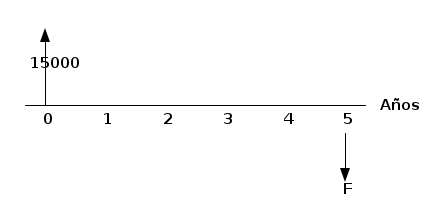
\includegraphics[width=10cm]{./img/incisoa.png}
\caption{i = 10\% anual}
\end{figure}


\begin{itemize}
\item b) La compañia ha decidido, hoy y en los proximos 4 años siguientes gastar \$50,000 en sistemas de seguridad se desea conocer la cantidad equivalente de estos gastos al final del cuarto año considerando una tasa del 12\% anual.
\end{itemize}

\begin{figure}[htbp]
\centering
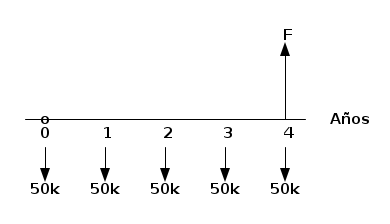
\includegraphics[width=10cm]{./img/incisob.png}
\caption{i = 12\% anual}
\end{figure}


\begin{itemize}
\item c) Un padre desea depositar una cantidad dentro de dos años. suficiente para retirar dentro de tres años 4000 anuales pos 5 años. Conciderando una tasa de interes del \%15.
\end{itemize}

\begin{center}
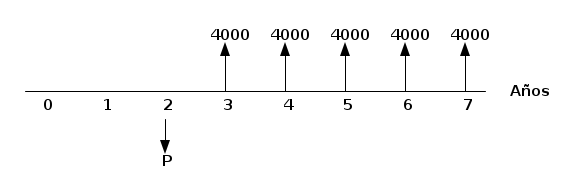
\includegraphics[width=.9\linewidth]{img/incisoc.png}
\end{center}


\begin{itemize}
\item d) Una empresa de alquiler de equipos gasto \$25,000 en una compresora hace 7 años. Por alquiler de la compresora, se obtiene un ingreso anual de \$7,500 los gastos de mantenimiento durante el primer año fueron de \$1,000 y aumentaron en \$250 cada año. La empresa desea vender la compresora por \$1,500 al final del proximo año.
\end{itemize}

\begin{figure}[htbp]
\centering
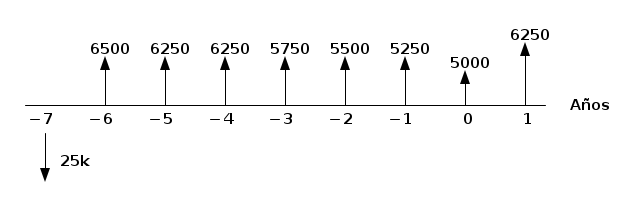
\includegraphics[width=10cm]{img/incisod.png}
\caption{insiso d}
\end{figure}

\subsection*{Desarrollo de la formula de interes compuesto}
\label{sec:orgec89424}
\begin{mdframed}
\[ \begin{aligned}
F_1 &= P(1+i) \\
F_2 &= F_1(1+i) = P(1+i)(1+i) = P(1+i)^2 \\
F_3 &= F_2(1+i) = P(1+i)(1+i)(1+i) = P(1+i)^3 
\end{aligned} \]

\begin{center}
\begin{tabular}{ll}
Futuro dado un presente & Presente dado un futuro\\
\(F = P(1+i)^n = P(F/P, i\%, n)\) & \(P = F \left[1/(1+i)^n\right] = F(p/f, i\%,n)\)\\
\end{tabular}

\end{center}
\end{mdframed}

\subsubsection*{Ejercicios}
\label{sec:orgc4f11aa}
\begin{itemize}
\item a) Una persona espera recibir una herencia dentro de 5 años por un total de \$50,000 si la tasa de interés es del 12\% cada año calcular la cantidad equivalente al día de hoy.
\end{itemize}

\begin{figure}[htbp]
\centering
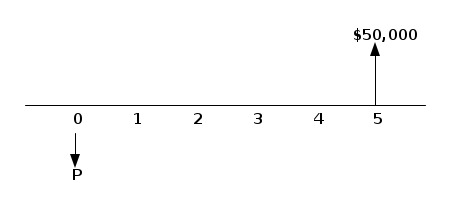
\includegraphics[width=.9\linewidth]{img/ejerccio1.png}
\caption{el valor P es igual a \$28,371.34}
\end{figure}

una herencia de \$50,000 en 5 años equivale actualmente a \$28,371.34 con una tasa del \%12.

\begin{itemize}
\item b) Un ingeniero resivio un bono de \$12,000 que desea invertir ahora. quiere calcular un valor equivalente despues de 24 años, cuando planea usar todo el dinero resultante como enganche para una casa. Suponga una tasa de retorno de 8\% durante los 24 años, calcular el monto que podra usar de enganche por la inversion.
\end{itemize}

\begin{figure}[htbp]
\centering
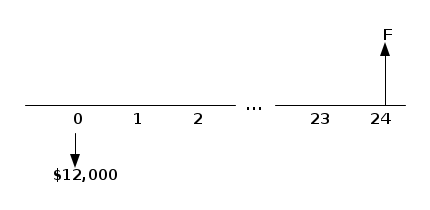
\includegraphics[width=.9\linewidth]{wdqweewq.png}
\caption{F es igual a \$76,094.17}
\end{figure}

Un inversion de \$12,000 hoy, generaria un monto de \$76,094.17 a 24 años considerando una tasa de rendimiento de 8\% en el futuro que podra utilizar en el enganche de la casa

\subsection*{Anualidad}
\label{sec:org7b989d0}
Es un \textbf{conjunto de pagos iguales realizados en intervalos iguales de tiempo}\footnote{estrictamente el concepto de anualidad proviene de años, pero en este caso llamaremos anualidad a todos los pagos realizados en intervalos iguales de tiempo.}. También se le conoce como serie uniforme, flujo constante, renta, mensualidad etc\ldots{} Ejemplos:

\begin{itemize}
\item Pagos mensuales por renta
\item Abonos a crédito
\item Pagos de sueldos
\end{itemize}

\subsubsection*{Ejercicio}
\label{sec:org88cb104}
¿Cuanto dinero se debe invertir hoy?, para que en cada año se retiren cada año \$600 durante los proximos 9 años, el inicio de los retiros comienza el proximo año suponer una tasa de rendimiento del 16\%

\begin{figure}[htbp]
\centering
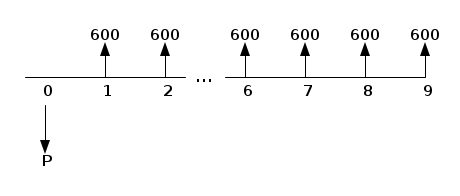
\includegraphics[width=.9\linewidth]{img/anualidad_1.png}
\caption{Presente dado una anualidad (\$2763.9263)}
\end{figure}

se debe invertir hoy 2763.9263 para cada año podamos retirar 600 cada año por los proximos 9 años a una tasa de 16\%

\subsubsection*{{\bfseries\sffamily TODO} Formula de la anualidad}
\label{sec:org514c862}
\[
 P = A\left[ \frac{1}{1+i} \right] + 
     A\left[ \frac{1}{(1+i)^2} \right] + 
     ... +
     A\left[ \frac{1}{(1+i)^{n-1}} \right] + 
     A\left[ \frac{1}{(1+i)^{n}} \right]  
\]

\[
 P = A\left[ \frac{1}{1+i} + \frac{1}{(1+i)^2} + 
     ... + \frac{1}{(1+i)^{n-1}} + \frac{1}{(1+i)^{n}} 
    \right]  
  \]

\[
\frac{1}{1+i} P = A\left[ \frac{1}{(1+i)^2} + \frac{1}{(1+i)^3} + 
     ... + \frac{1}{(1+i)^{n-1}} + \frac{1}{(1+i)^{n}} 
    \right]  
\]


Presente dado una anualidad:
\[
xP = A\frac{(1+i)^n-1}{i(1+i)^n} = A(P/A, i\%, n)
\]


Anualidad dada un presente:
\[
A = P\frac{i(1+i)^n}{(1+i)^n-1} = P(A/P, i\%, n)
\]

\subsubsection*{{\bfseries\sffamily TODO} Ejericio 2}
\label{sec:org47ca16d}
Una empresa requiere de un equipo para producir que cuesta \$3,400,000. La empresa espera tener una tasa de rendimiento del 20\% y recuperar su inversion dentro de 8 años. ¿Cual debe ser la ganacia total neta?

\begin{center}
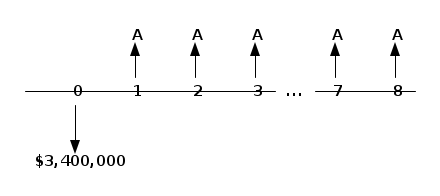
\includegraphics[width=.9\linewidth]{fgabvcvn.png}
\end{center}


por 8 años se esperan ganacias de \$886,072.04 para recupera la inversion para la compra del equipo de produccion  

\subsubsection*{{\bfseries\sffamily TODO} Futuro dado una anualidad}
\label{sec:orgbd1acc8}
\[ F=A\left[\frac{(1+i)^n-1}{i}\right] = A(F/A, i\%, n) \]

\subsubsection*{{\bfseries\sffamily TODO} Anualidad dado un futuro}
\label{sec:orgbc75efc}
\subsubsection*{Ejercicio}
\label{sec:org69c0eab}
\begin{itemize}
\item el presidente de una compañia desea saber el valor futuro equivalente de una inversion por un millon por cada año por 8 años emepzando el proximo año, la inversion gana una tasa de 14\% al año
\end{itemize}

\begin{mdframed}
por una inversion de 1 millon anual por 8 años es equivalente a \$13,232760.16 en el octavo año con una tasa de \%14
\end{mdframed}

\begin{itemize}
\item ¿cuanto dinero se encesita depositar cada año?, para que se pueda acumular 6000 en 7 años con una tasa de interes de 5.5\% por año y los depositos inician el proximo año
\end{itemize}

\begin{mdframed}
cada año necesia depocitar 725.79 cada año por 7 años para acumular cantidad de \$6000 en 7 años considerando una tasa de 5.5\%
\end{mdframed}

\subsection*{Gradiente aritmetico}
\label{sec:org4547f1a}
Es el cambio aritmetico de margnitud constante, ya sea por ingresos o desembolsos, de un periodo al siguiente el gradiente aritmetico se calcula:

\[
G = \frac{C_n - CB}{n-1}
\]

\begin{description}
\item[{C\_n}] es la cantidad en el periodo n
\item[{CB}] cantidad Base
\end{description}

\subsubsection*{Presente dado un gradiente}
\label{sec:org0c48ec0}

\[
P_G = G\left[ \frac{ (1+i)^n - in-1 }{ i^2 (1+i)^n } \right] = G(p/g, i\%, n)
\]

\subsubsection*{Anualidad dado un gradiente}
\label{sec:orgb597956}
\[
P =A\left[ \frac{(1+i)^n - 1}{i(1+i)^n} \right]
\]

\[
A_G = \left[ \frac{(1+i)^n-1}{i(1+i)^n} \right]= G \left[ \frac{(1+i)^n-i\cdot n-1}{i^2 (1+i)^n} \right]
\]

\[
A_G\left[ (1+i)^n-1 \right] = G\left[ \frac{(1+i)^n - in-1}{i^2(1+i)^n} \right] (i(1+i)^n)
\]

\[
A_G\left[(1+i)^n-1\right] = G\left[ \frac{(1+i)^n - in - 1}{i} \right]
\]


\[
A_G = \frac{G}{i} [ \frac{ (1+i)^n - 1 - in }{ (1+i)^n - 1} ]
\]

\[
A_G= \frac{G}{i} [ 1 - \frac{in}{ (1+i)^n - 1} ]
\]

\[
A_G = G \left[ \frac{1}{i} - \frac{n}{(1+i)^n-1}\right] = G(A/G,i\%,n) 
\]

\subsubsection*{Futuro dado un gradiente}
\label{sec:org8bd4e4c}

\[
F_G = \left[ \frac{1}{(1+i)^n} \right] = G\left[ \frac{(1+i)^n-in-1}{i^2(1+i)^n} \right]
\]

\[
F_G = G\left[ \frac{(1+n)^n - in - 1}{i^2(1+i)^n} \right] (1+i)^n
\]

\[
F_G = G \left[ \frac{(1+i)^n - in - 1}{i^2} \right]
\]

\[
F_G = G \left[ (\frac{1}{i}) (\frac{(1+i)^n-1}{i} - n) \right] = G(F/G,i\%, n)
\]


presentes

P = P\_A + P\_G : gradiente cresiente
P = P\_A - P\_G: gradiente decresiente

futuros

F = F\_A + F\_G : gradiente cresiente
F = F\_A - F\_G : gradiente decresiente

Anualidad del gradiente

A = CB + A\_G 


para determinar el valor presente total (P) para una serie de gradiente se debe considerar tanto el valor presente de la anualidad de la serie de gradiente como el valor presente del valor del gradiente.

\subsubsection*{Ejercicio 1}
\label{sec:org8188701}
Se ha acordado ahorrar recursos para mantenimiento de infraestructura. En el primer año se depositara \$500,000 que aumentarán en \$100,000 para los siguentes 9 años, calcule el valor presente con una tasa de interes del 5\%:

\begin{center}
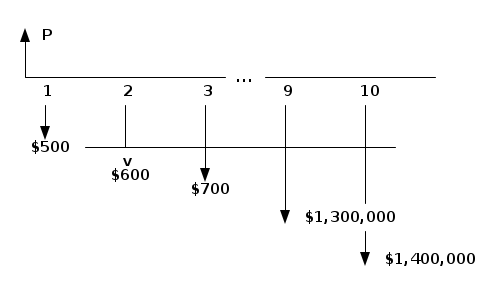
\includegraphics[width=.9\linewidth]{fsdfds.png}
\end{center}



Presente dado un gradiente

\[
P_G = 100,000 [ ((1+0.05)^{10} - 0.05*10 - 1) / ((0.05)^2 (1+0.05)^{10} ) ] = \$3165204.79
\]

\[
P_A =500,000 [ ((1+0.05)^{10} - 1) / ((0.05)(1+0.05)^{10}) ] = \$3860867.47
\]

\[
\$3165204.79 + \$3860867.47 = \$7,026,072.25
\]

el valor presente de todos los depositos que se van a hacer durante los proximos 10 años es de \$7,026,072.25.

\subsubsection*{Ejercicio 2}
\label{sec:orgad48a74}
Con la implementacion de una nueva maquinaria de produccion, se espera ingresos en el primer año por \$280,000. Tambien se piensa que estos ingresos disminuiran deacuerdo con un gradiente arimetico de \$50,000 por año. Cual es el valor anual uniforme de estos ingresos en 5 años con una tasa anual de 12\%.

\$280   
 \^{}    \$230 
\begin{center}
\begin{tabular}{l}
\^{}    \$180\\
 & \^{}    \$130\\
 &  & \^{}    \$80\\
 &  &  & \^{}\\
 &  &  & \\
\end{tabular}

\end{center}
--\sout{-----}-----\sout{-----}-----+--

anualidad dado un gradiente (gradiente decreciente):

50,000 * ( 1/0.12 - 5/((1+0.12)\^{}5 - 1) ) = \$88729.72512

A = 280,000 - 88729.72512 = 191270.2749

A = CB - A\_G

el valor anual de estos ingresos a 5 años es de \$191,270.2749 con una tasa de interes del 12\%

\section*{{\bfseries\sffamily TODO} tasa de interes y periodos desconocidos}
\label{sec:orge0cc154}
en algunos casos, para encontrar i o n desconocidos sera necesario interpolar utilizando las tablas de factores.

\section*{ejercio 1}
\label{sec:org96232a5}
encuanto tiempo se triplicara 1000, si la tasa de interes es de 10\% anual

\section*{{\bfseries\sffamily TODO} ejercicio 2}
\label{sec:org07a1148}
\end{document}
